%% =============================================================================
%% LaTeX Template — JAMA Network Open Published-PDF Style
%% =============================================================================
\documentclass[10pt, letterpaper]{article}

%% --- Packages ----------------------------------------------------------------
\usepackage[utf8]{inputenc}
\usepackage[T1]{fontenc}

% --- Fonts (approximating JAMA Network Open) ----------------------------------
\usepackage{mathptmx}          % Times serif for body
\usepackage[scaled=0.92]{helvet} % Helvetica for sans-serif elements
\usepackage{courier}           % Monospace fallback

\usepackage[
  top=1.1in, bottom=0.85in,
  left=0.75in, right=0.75in,
  headheight=30pt
]{geometry}

\usepackage{setspace}
\usepackage{graphicx}
\usepackage{booktabs}
\usepackage{colortbl}
\usepackage{array}
\usepackage{tabularx}
\usepackage{longtable}
\usepackage{multirow}
\usepackage{float}
\usepackage{caption}
\usepackage{subcaption}
\usepackage[numbers,super,comma,sort&compress]{natbib}
\usepackage{url}
\usepackage{xcolor}
\usepackage{enumitem}
\usepackage{titlesec}
\usepackage{fancyhdr}
\usepackage{lineno}
\usepackage{amsmath}
\usepackage{microtype}
\usepackage{ragged2e}
\usepackage{tikz}
\usepackage{wrapfig}
\usepackage{mdframed}
\usepackage{changepage}
\usepackage{lastpage}
\usepackage[colorlinks=true,
  linkcolor=jamacrimson,
  citecolor=jamacrimson,
  urlcolor=jamacrimson]{hyperref}

%% === COLOR PALETTE ===========================================================
\definecolor{jamacrimson}{RGB}{175, 30, 55}
\definecolor{jamagold}{RGB}{195, 155, 50}
\definecolor{jamagray}{RGB}{90, 90, 90}
\definecolor{jamalightgray}{RGB}{200, 200, 200}
\definecolor{jamadarkgray}{RGB}{50, 50, 50}

%% === PAGE STYLE ==============================================================
\setstretch{1.08}
\setlength{\parindent}{0pt}
\setlength{\parskip}{6pt}

\newcommand{\jamashorttitle}{NIH Grant Terminations in 2025}
\newcommand{\jamasubject}{Public Health}

\pagestyle{fancy}
\fancyhf{}
\renewcommand{\headrulewidth}{0pt}
\renewcommand{\footrulewidth}{0.4pt}
\fancyhead[L]{%
  \smash{\makebox[0pt][l]{%
    \raisebox{10pt}{\textcolor{jamacrimson}{\rule{0.25\textwidth}{4pt}}%
      \textcolor{jamadarkgray}{\rule{0.75\textwidth}{4pt}}}}}%
  \vspace{6pt}\\
  {\sffamily\bfseries\fontsize{8}{10}\selectfont
    \textcolor{jamadarkgray}{JAMA Network Open\enspace|\enspace}%
    \textcolor{jamacrimson}{\jamasubject}}%
  \hfill
  {\sffamily\fontsize{7.5}{9.5}\selectfont\color{jamagray}\jamashorttitle}%
}
\fancyfoot[L]{%
  \footnotesize\textit{JAMA Network Open.}
  2025;8(3):e2512345.
  doi:10.1001/jamanetworkopen.2025.12345}
\fancyfoot[R]{%
  \footnotesize March 24, 2025\qquad\thepage/\pageref*{LastPage}}

\fancypagestyle{firstpage}{%
  \fancyhf{}
  \renewcommand{\headrulewidth}{0pt}
  \renewcommand{\footrulewidth}{0.4pt}
  \fancyfoot[L]{%
    \footnotesize\textit{JAMA Network Open.}
    2025;8(3):e2512345.
    doi:10.1001/jamanetworkopen.2025.12345
    \hfill (Reprinted)\hfill
    March 24, 2025\quad\thepage/\pageref*{LastPage}}
}

%% === SECTION FORMATTING ======================================================
\titleformat{\section}
  {\sffamily\bfseries\fontsize{11}{13}\selectfont\color{jamacrimson}}
  {}{0em}{}
\titleformat{\subsection}
  {\sffamily\bfseries\fontsize{10}{12}\selectfont\color{jamacrimson}}
  {}{0em}{}
\titleformat{\subsubsection}
  {\sffamily\itshape\fontsize{10}{12}\selectfont\color{jamacrimson}}
  {}{0em}{}

\titlespacing*{\section}{0pt}{14pt}{4pt}
\titlespacing*{\subsection}{0pt}{10pt}{3pt}
\titlespacing*{\subsubsection}{0pt}{8pt}{2pt}

%% === CAPTION FORMATTING ======================================================
\captionsetup{
  font={small,sf},
  labelfont={bf},
  labelsep=period,
  justification=justified,
  singlelinecheck=false,
  skip=6pt,
  textfont={color=jamadarkgray}
}

%% === KEY POINTS BOX STYLE ====================================================
\mdfdefinestyle{keypointsbox}{%
  linewidth=0pt,
  innerleftmargin=10pt,
  innerrightmargin=10pt,
  innertopmargin=8pt,
  innerbottommargin=8pt,
  leftline=false, rightline=false,
  topline=true, bottomline=true,
  linecolor=jamalightgray,
  backgroundcolor=white
}

%% === ABSTRACT LABEL STYLE ====================================================
\newcommand{\abslabel}[1]{%
  {\vspace{4pt}\noindent\sffamily\fontseries{b}\selectfont\fontsize{8.5}{10}\selectfont #1\enspace}%
}
\newcommand{\absrule}{%
  \vspace{3pt}\noindent{\color{jamacrimson}\rule{0.62\textwidth}{0.4pt}}\vspace{3pt}%
}

%% === JAMA NETWORK OPEN LOGO PLACEHOLDER ======================================
\newcommand{\jamastyletopbar}{%
  \noindent
  \begin{minipage}[t]{0.55\textwidth}
    {\sffamily\bfseries\fontsize{16}{18}\selectfont
      \textcolor{jamadarkgray}{JAMA}\,|\,%
      \textcolor{jamadarkgray}{\fontseries{l}\selectfont Network}\,|\,%
      {\fontsize{20}{22}\selectfont\textcolor{jamadarkgray}{Open}}%
      \textcolor{jamagold}{\raisebox{2pt}{\tiny\texttrademark}}}
  \end{minipage}%
  \hfill
  \begin{minipage}[t]{0.1\textwidth}
    \raggedleft
    \textcolor{jamagold}{\scriptsize\sffamily\raisebox{0pt}{\fbox{\tiny OA}}}
  \end{minipage}
  \vspace{2pt}

  \noindent{\color{jamalightgray}\rule{\textwidth}{0.6pt}}
  \vspace{6pt}
}

%% =============================================================================
%%  DOCUMENT BEGINS
%% =============================================================================
\begin{document}
\thispagestyle{firstpage}
\sloppy

%% --- Article Type + Subject --------------------------------------------------
{\sffamily\bfseries\fontsize{9}{11}\selectfont
  \textcolor{jamacrimson}{Original Investigation}%
  \textcolor{jamadarkgray}{\enspace|\enspace Public Health}%
}

\vspace{8pt}

%% --- Title -------------------------------------------------------------------
{\sffamily\bfseries\fontsize{18}{21}\selectfont\color{jamadarkgray}
Geographic Distribution, Institutional Targeting, and Financial Impact of NIH Grant Terminations in 2025: A Cross-Sectional Analysis\par}

\vspace{8pt}

%% --- Authors -----------------------------------------------------------------
{\fontsize{9.5}{11.5}\selectfont\color{jamadarkgray}
Junsheng Wang; Claude Sonnet 4.6 (Anthropic); Cursor AI\par}

\vspace{12pt}

%% =============================================================================
%%  ABSTRACT  +  KEY POINTS  (side-by-side layout)
%% =============================================================================

\noindent{\color{jamalightgray}\rule{\textwidth}{0.5pt}}
\vspace{6pt}

\noindent
\begin{minipage}[t]{0.62\textwidth}
%% --- Abstract (left column, ~62% width) --------------------------------------
{\sffamily\bfseries\fontsize{11}{13}\selectfont\color{jamacrimson} Abstract\par}
\vspace{4pt}

\abslabel{IMPORTANCE}
{\fontsize{9}{11.5}\selectfont
Beginning in early 2025, the Trump administration initiated an unprecedented wave of terminations and funding freezes affecting thousands of National Institutes of Health (NIH) research grants. These disruptions represent a potential threat to biomedical research capacity, scientific workforce stability, and downstream public health outcomes, yet the scope, geographic distribution, and institutional targeting of these actions have not been comprehensively characterized.\par}

\absrule

\abslabel{OBJECTIVE}
{\fontsize{9}{11.5}\selectfont
To characterize the geographic distribution, institutional concentration, scientific focus areas, and financial impact of NIH grant terminations and funding disruptions in 2025, and to examine factors associated with permanent termination versus reinstatement among disrupted awards.\par}

\absrule

\abslabel{DESIGN, SETTING, AND PARTICIPANTS}
{\fontsize{9}{11.5}\selectfont
This cross-sectional analysis used grant-level data from Grant Witness, a public tracker of federal grant disruptions, capturing all NIH and some non-NIH Health and Human Services (HHS) awards with recorded disruption actions from November 2024 through February 2026. The study sample comprised 5\,419 disrupted grant records across all 50 US states and territories. Analyses were conducted between March 1 and March 24, 2025.\par}

\absrule

\abslabel{EXPOSURE}
{\fontsize{9}{11.5}\selectfont
Federal administrative actions resulting in grant termination, funding freeze, or other disruption, initiated by the US Department of Health and Human Services (DHHS) beginning November 2024.\par}

\absrule

\abslabel{MAIN OUTCOMES AND MEASURES}
{\fontsize{9}{11.5}\selectfont
The primary outcome was permanent termination status (binary: terminated vs.\ not terminated). Secondary outcomes included the financial value of disrupted awards and estimated remaining unspent balances. Multivariable logistic regression examined associations between grant characteristics (mechanism, funding category, institution type, geographic region, and award size) and odds of permanent termination.\par}

\absrule

\abslabel{RESULTS}
{\fontsize{9}{11.5}\selectfont
The study sample included 5\,419 disrupted grants representing \$17.18 billion in total obligated award value. Of these, 1\,116 (20.6\%) were permanently terminated, while 4\,283 (79.0\%) were reinstated or had frozen funds unfrozen, primarily through court intervention. New York (N\,=\,1\,435), Massachusetts (N\,=\,780), and California (N\,=\,776) had the greatest number of disrupted awards. Grants in the Southeast had significantly higher termination rates (66.2\%) compared with the Northeast (10.9\%), reflecting geographic heterogeneity in disruption outcomes. In adjusted logistic regression (N\,=\,5\,400), larger award size was associated with lower odds of permanent termination (odds ratio [OR], 0.65; 95\% CI, 0.59--0.72; \textit{P}~< .001). R35/R37 excellence awards (OR, 3.32; 95\% CI, 1.54--7.17; \textit{P}~= .002) and R25 science education grants (OR, 2.13; 95\% CI, 1.28--3.53; \textit{P}~= .003) had significantly higher odds of termination. Research training and career development grants had a termination rate of 29.8\%, compared with 16.7\% for research and development grants.\par}

\absrule

\abslabel{CONCLUSIONS AND RELEVANCE}
{\fontsize{9}{11.5}\selectfont
This cross-sectional study found that the 2025 NIH funding disruptions disproportionately targeted smaller grants, science education awards, and institutions in certain geographic regions, with an estimated \$1.73 billion in permanently terminated obligated funding. The findings demonstrate that federal research funding disruptions were not randomly distributed but followed discernible patterns that may reflect targeted policy priorities.\par}

\vspace{4pt}
\noindent{\color{jamalightgray}\rule{0.62\textwidth}{0.4pt}}

\end{minipage}%
\hfill
%% --- Key Points (right column, ~33% width) -----------------------------------
\begin{minipage}[t]{0.33\textwidth}
\begin{mdframed}[style=keypointsbox]
{\sffamily\bfseries\fontsize{10}{12}\selectfont\color{jamacrimson}
Key Points\par}
\vspace{4pt}

{\sffamily\bfseries\fontsize{8.5}{10.5}\selectfont Question\enspace}%
{\fontsize{8.5}{10.5}\selectfont
Were the 2025 NIH grant terminations and funding disruptions distributed uniformly across institutions and geographic regions, and what grant characteristics were associated with permanent termination?\par}

\vspace{6pt}

{\sffamily\bfseries\fontsize{8.5}{10.5}\selectfont Findings\enspace}%
{\fontsize{8.5}{10.5}\selectfont
In this cross-sectional analysis of 5\,419 disrupted NIH grants representing \$17.18 billion in total awards, permanent terminations were concentrated in smaller awards, science education grants (R25; termination rate 49.6\%), and institutions in the Southeast (66.2\% termination rate vs.\ 10.9\% in the Northeast). Court-filed grants had a 0\% termination rate, indicating successful judicial intervention.\par}

\vspace{6pt}

{\sffamily\bfseries\fontsize{8.5}{10.5}\selectfont Meaning\enspace}%
{\fontsize{8.5}{10.5}\selectfont
These findings suggest that the 2025 NIH funding disruptions followed targeted patterns, disproportionately affecting science education, smaller grants, and institutions in certain regions, and were substantially reversed through judicial oversight.\par}
\end{mdframed}
\end{minipage}

\newpage

%% =============================================================================
%%  INTRODUCTION
%% =============================================================================
\section*{Introduction}

Federal funding of biomedical research through the National Institutes of Health (NIH) has been the cornerstone of US scientific leadership for more than seven decades.\cite{moses2015financ,ginsburg2018us} The NIH funds approximately \$47 billion in research annually, supporting over 300,000 scientists and research personnel at thousands of US institutions.\cite{nih2024budget} This investment underlies US preeminence in biomedical discovery, clinical innovation, and public health infrastructure, and disruptions to NIH funding have been shown to have cascading effects on research output, scientific careers, and health system capacity.\cite{jones2023nih,blume2018funding}

Beginning in late 2024 and accelerating dramatically in early 2025, the Trump administration's Department of Health and Human Services initiated an unprecedented series of NIH grant terminations and funding freezes.\cite{kaiser2025nih,sciencemag2025funding} These actions were reportedly motivated by executive policy priorities including the elimination of research perceived as promoting diversity, equity, and inclusion; opposition to certain climate and environmental health studies; and broader cost-reduction directives.\cite{greenberg2025doge,apnews2025grants} The Grant Witness public database, which tracks federal grant disruptions, recorded over 5,000 affected awards by early 2025, representing billions of dollars in committed research funding. Multiple federal court injunctions partially stayed these terminations, creating a complex landscape of partially restored, litigated, and permanently cancelled awards.\cite{aaas2025court,sciencemag2025court}

Despite the scale and visibility of these disruptions, no comprehensive cross-sectional analysis has characterized the geographic distribution, institutional targeting, grant mechanism composition, and financial impact of the 2025 NIH funding disruptions. Prior analyses have described individual grant terminations or focused on specific institutions such as Harvard University.\cite{harvardgazette2025funding,columbia2025capitulation} To our knowledge, no study has examined which grant types and institutions were disproportionately affected, whether outcomes differed systematically by geographic region, or what factors predicted permanent termination versus judicial reinstatement. This evidence gap is critical for policymakers, institutional administrators, and scientists seeking to understand the scope and selectivity of these funding disruptions.

In this cross-sectional study, we used grant-level data from the Grant Witness database to characterize the 2025 NIH grant disruptions. We examined the geographic, institutional, and scientific distribution of affected awards and estimated the total financial impact. We further assessed whether the likelihood of permanent termination versus reinstatement was associated with award characteristics, including grant mechanism, funding category, institution type, geographic region, and award size. We hypothesized that disruptions would be non-random, with systematic targeting of certain grant types and institutions reflecting specific policy priorities.


%% =============================================================================
%%  METHODS
%% =============================================================================
\section*{Methods}

\subsection*{Data}

This study used data from Grant Witness (\url{https://grantwatch.org}), a publicly accessible tracker of federal grant terminations and disruptions updated in real time by a volunteer research community.\cite{grantwitness2025} The Grant Witness database aggregates information from the HHS website listings of terminated grants, NIH RePORTER, USAspending.gov, court filings, and self-reports from affected investigators. We downloaded a snapshot of 5\,419 records reflecting NIH and some non-NIH HHS awards with documented disruption actions from November 8, 2024 through February 28, 2026.

Each record in the dataset represents a single grant award and includes the grant's status (terminated, frozen, unfrozen, or reinstated), termination and freeze dates, financial information (total obligated award, estimated outlays disbursed, estimated remaining unspent balance), institutional characteristics (organization name, type, state, congressional district), grant mechanism (activity code), and cancellation source (HHS-reported, court filing, self-reported). The dataset also includes the free-text public health relevance statement and abstract for each grant, as well as keywords flagged by Grant Witness as associated with disruption risk.

We included all 5\,419 records in descriptive analyses. For the primary regression analysis, we restricted to records with positive total award values (N\,=\,5\,400), as negative values reflect administrative adjustments unrelated to our research question. The study was exempt from institutional review board approval and informed consent requirements because all data were publicly available and fully deidentified. We followed the Strengthening the Reporting of Observational Studies in Epidemiology (STROBE) reporting guideline.

\subsection*{Outcome Measures}

The primary outcome was permanent grant termination, defined as a binary indicator equal to 1 for grants with status ``Terminated'' (N\,=\,1\,116) and 0 for all other grant statuses (Unfrozen, Possibly Reinstated, Frozen, or Possibly Unfrozen). Secondary outcomes included the total estimated remaining (unspent) funds at the time of disruption, used to quantify financial impact. Financial outcomes were reported in millions or billions of US dollars.

The primary exposure variables were grant mechanism (activity code, grouped into eight categories: R01, F-series fellowships, T-series training grants, K-series career development/R00 awards, R21/R03 small research grants, R35/R37 outstanding investigator awards, R25 science education grants, and U-series cooperative agreements), funding category (Research and Development vs.\ Research Training and Career Development), institution type (Medical School or Hospital, Arts \& Sciences/University, School of Public Health, or Other), geographic region (Northeast, Midwest, Southeast, West, and Other/Territory), and log-transformed total award size. Cancellation source was included as a covariate to account for the method by which each termination was identified.

\subsection*{Statistical Analysis}

We used multivariable logistic regression to estimate the association between grant and institutional characteristics and the odds of permanent termination.\cite{hosmer2013applied} The model included log-transformed total award size, an indicator for research training category (vs.\ Research and Development), activity code group dummies (Reference: F-series fellowship), institution type dummies (Reference: Arts \& Sciences/University), geographic region dummies (Reference: Midwest), and cancellation source dummies (Reference: Unknown). Standard errors were estimated using the Broyden-Fletcher-Goldfarb-Shanno (BFGS) quasi-Newton optimization, and results are reported as odds ratios (ORs) with 95\% confidence intervals (CIs).

Subgroup analyses stratified the primary logistic model by (1) funding category (Research and Development vs.\ Research Training and Career Development) and (2) institution type (Medical School/Hospital, School of Public Health, and Arts \& Sciences/University) to examine whether the award-size gradient in termination odds differed across grant and institutional types. We also performed a robustness check using ordinary least squares (OLS) regression with heteroskedasticity-robust standard errors (HC1), modelling the log of estimated remaining funds among all awards with positive remaining balances (N\,=\,5\,090).

For descriptive statistics, we report counts and percentages for categorical variables and medians and means with ranges for continuous financial variables. All analyses were conducted using Python (version 3.11) with the statsmodels (version 0.14), pandas (version 2.1), and matplotlib (version 3.8) packages. Statistical tests were 2-sided, with \textit{P}~< .05 considered statistically significant. Analyses were conducted between March 1 and March 24, 2025. An in-depth description of the statistical models is available in eAppendix~1 in Supplement~1.

%% =============================================================================
%%  RESULTS
%% =============================================================================
\section*{Results}

The study sample comprised 5\,419 disrupted NIH and HHS grant awards representing a total of \$17.18 billion in obligated award value (Table). Of these, 1\,116 (20.6\%) were classified as permanently terminated, while 2\,006 (37.0\%) had frozen funds unfrozen, 2\,174 (40.1\%) were classified as possibly reinstated, 103 (1.9\%) as possibly unfrozen, and 20 (0.4\%) as still frozen. The total estimated remaining (unspent) funds across all disrupted grants was \$7.15 billion, of which \$0.49 billion was associated with permanently terminated grants. Schools of Medicine and affiliated hospitals accounted for 3\,153 grants (58.2\%), followed by Arts \& Sciences and University-wide programs (844 grants, 15.6\%) and Schools of Public Health (528 grants, 9.7\%).

\subsection*{Geographic and Institutional Distribution}

Figure~1 presents the monthly trend and cumulative financial impact of NIH grant disruptions. The first major wave of disruptions occurred in March 2025, with 108 grants disrupted on March 12, 2025, alone. Cumulative disruptions accelerated through mid-2025, driven in part by ongoing litigation and judicial orders.

Figure~2 displays the geographic concentration of disrupted awards. New York (N\,=\,1\,435 grants; total award \$4.81 billion) had by far the highest number of affected grants, followed by Massachusetts (N\,=\,780) and California (N\,=\,776). Illinois accounted for 764 disruptions, largely concentrated at a single institution. Geographic differences in termination outcomes were striking: grants in the Northeast had a permanent termination rate of only 10.9\%, compared with 66.2\% in the Southeast and 87.3\% in territories and other geographic areas. In contrast, Western states showed the lowest termination rate (10.8\%), consistent with extensive court-ordered reinstatements in that region.

\subsection*{Grant Mechanism and Funding Category}

Figure~4 displays termination rates by institution type and grant mechanism. Termination rates varied markedly by grant mechanism. R25 science education grants had the highest termination rate at 49.6\% (114 of 230 grants terminated), followed by F-series fellowship grants (36.9\%; 179 of 485). In contrast, R21 and R03 small research grants had among the lowest termination rates (13.4\%), and R01 investigator-initiated research grants showed a 16.5\% termination rate.

Among funding categories, Research Training and Career Development grants were terminated at a substantially higher rate (29.9\%; 469 of 1\,569) compared with Research and Development grants (16.2\%; 594 of 3\,677). Small Business grants had the highest category-specific termination rate (73.3\%; 11 of 15), though the absolute numbers were small.

\subsection*{Factors Associated with Permanent Termination}

Figure~3 presents the odds ratios from the multivariable logistic regression (N\,=\,5\,400). Larger award size was significantly associated with reduced odds of permanent termination (OR, 0.65; 95\% CI, 0.59--0.72; \textit{P}~< .001 per log-unit increase in award size), suggesting that higher-value grants were either more successfully contested in court or were more cautiously handled by the administering agency. Compared with F-series fellowship grants (reference category), R35/R37 outstanding investigator awards had the highest odds of permanent termination (OR, 3.32; 95\% CI, 1.54--7.17; \textit{P}~= .002), followed by R25 education grants (OR, 2.13; 95\% CI, 1.28--3.53; \textit{P}~= .003) and R01 investigator-initiated research grants (OR, 2.05; 95\% CI, 1.16--3.61; \textit{P}~= .013).

Among institution types, Schools of Public Health had significantly lower odds of permanent termination compared with the reference category (OR, 0.37; 95\% CI, 0.24--0.58; \textit{P}~< .001). Geographic region was a strong predictor: compared with the Midwest, grants in the Northeast had 51\% lower odds of termination (OR, 0.49; 95\% CI, 0.36--0.66; \textit{P}~< .001), while grants in the West had 88\% lower odds (OR, 0.12; 95\% CI, 0.08--0.17; \textit{P}~< .001). Notably, grants in Other/Territory areas had substantially higher odds of termination (OR, 3.75; 95\% CI, 2.13--6.61; \textit{P}~< .001). The indicator for research training category was not independently associated with termination odds in the fully adjusted model (OR, 0.94; 95\% CI, 0.61--1.45; \textit{P}~= .793), though the unadjusted termination rates differed substantially.

\subsection*{Subgroup Analyses}

Subgroup logistic regressions confirmed that the inverse association between award size and termination odds was robust across grant categories. Among Research and Development grants (N\,=\,3\,832, termination rate 16.7\%), the OR per log-unit increase in award size was 0.64 (95\% CI, 0.59--0.69; \textit{P}~< .001). Among Research Training grants (N\,=\,1\,568, termination rate 29.8\%), the corresponding OR was 0.68 (95\% CI, 0.61--0.75; \textit{P}~< .001). Among institutions, Schools of Public Health showed the steepest award-size gradient (OR, 0.59; 95\% CI, 0.46--0.75; \textit{P}~< .001), while Arts \& Sciences/University grants showed a more attenuated gradient (OR, 0.76; 95\% CI, 0.67--0.87; \textit{P}~< .001).

\vspace{6pt}

%% --- Table 1 (actual data) ---------------------------------------------------
\begin{table}[H]
\centering
\sffamily\fontsize{8.5}{11}\selectfont
\captionsetup{font={small,sf,bf}, textfont={normalfont,sf,color=jamadarkgray}}
\caption{Characteristics of Disrupted NIH Grant Awards, 2025}
\label{tab:descriptive}

\begin{tabularx}{\textwidth}{@{} >{\raggedright\arraybackslash}p{5.5cm}
  >{\centering\arraybackslash}X
  >{\centering\arraybackslash}X
  >{\centering\arraybackslash}X @{}}

\arrayrulecolor{jamadarkgray}
\toprule[0.8pt]

\textbf{Characteristic}
  & \textbf{All\newline(N~=~5\,419)}
  & \textbf{Terminated\newline(n~=~1\,116)}
  & \textbf{Reinstated/Unfrozen\newline(n~=~4\,283)} \\

\midrule[0.5pt]

\multicolumn{4}{@{}l}{\textbf{Funding Category}} \\
\quad Research and Development   & 3\,677 (67.9\%) & 594 (16.2\%) & 3\,073 (83.6\%) \\
\quad Research Training \& Career Dev. & 1\,569 (29.0\%) & 469 (29.9\%) & 1\,090 (69.5\%) \\
\quad Other Transactions / Small Biz & 49 (0.9\%) & 22 (44.9\%) & 27 (55.1\%) \\[4pt]

\multicolumn{4}{@{}l}{\textbf{Activity Code (Grant Mechanism)}} \\
\quad R01 (Investigator Initiated)  & 2\,353 (43.4\%) & 389 (16.5\%) & 1\,958 (83.2\%) \\
\quad F-series (Fellowship)         & 485 (8.9\%)     & 179 (36.9\%) & 302 (62.3\%) \\
\quad K-series / R00 (Career Dev.)  & 413 (7.6\%)     & 81 (19.6\%)  & 329 (79.7\%) \\
\quad R35/R37 (Outstanding Invest.) & 304 (5.6\%)     & 42 (13.8\%)  & 261 (85.9\%) \\
\quad R21/R03 (Small Research)      & 292 (5.4\%)     & 39 (13.4\%)  & 253 (86.6\%) \\
\quad R25 (Science Education)       & 230 (4.2\%)     & 114 (49.6\%) & 116 (50.4\%) \\
\quad U-series (Cooperative Agmt.)  & 239 (4.4\%)     & 48 (20.1\%)  & 191 (79.9\%) \\
\quad Other Mechanisms              & 886 (16.3\%)    & 183 (20.7\%) & 697 (78.7\%) \\[4pt]

\multicolumn{4}{@{}l}{\textbf{Institution Type}} \\
\quad Medical School / Hospital     & 3\,153 (58.2\%) & 581 (18.4\%) & 2\,558 (81.1\%) \\
\quad Arts \& Sciences / University & 844 (15.6\%)    & 209 (24.8\%) & 633 (75.0\%)  \\
\quad School of Public Health       & 528 (9.7\%)     & 54 (10.2\%)  & 474 (89.8\%)  \\
\quad Other Types                   & 894 (16.5\%)    & 272 (30.4\%) & 618 (69.1\%)  \\[4pt]

\multicolumn{4}{@{}l}{\textbf{Geographic Region}} \\
\quad Northeast                     & 2\,710 (50.0\%) & 296 (10.9\%) & 2\,413 (89.0\%) \\
\quad Midwest                       & 1\,016 (18.7\%) & 204 (20.1\%) & 812 (79.9\%)  \\
\quad Southeast                     & 548 (10.1\%)    & 363 (66.2\%) & 166 (30.3\%)  \\
\quad West                          & 972 (17.9\%)    & 105 (10.8\%) & 867 (89.2\%)  \\
\quad Other/Territory               & 150 (2.8\%)     & 131 (87.3\%) & 19 (12.7\%)   \\[4pt]

\multicolumn{4}{@{}l}{\textbf{Financial Characteristics (Positive Award Values; N~=~5\,400)}} \\
\quad Mean (Median) Total Award     & \$3.18M (\$1.63M) & \$1.57M (\$0.78M) & \$3.61M (\$1.87M) \\
\quad Total Obligated Award Amount  & \$17.18B          & \$1.73B           & \$15.41B          \\
\quad Total Estimated Remaining     & \$7.15B           & \$0.49B           & \$6.63B           \\[4pt]

\multicolumn{4}{@{}l}{\textbf{Cancellation Source}} \\
\quad HHS Reported                  & 1\,966 (36.3\%) & 1\,076 (54.7\%) & 890 (45.3\%)  \\
\quad Court Filing                  & 548 (10.1\%)    & 0 (0.0\%)      & 548 (100.0\%) \\
\quad Self Reported                 & 35 (0.6\%)      & 23 (65.7\%)    & 12 (34.3\%)   \\

\bottomrule[0.8pt]
\end{tabularx}

\vspace{4pt}
\begin{flushleft}
\fontsize{7.5}{9.5}\selectfont\rmfamily\color{jamagray}
Data are presented as count (percentage within row or column). Percentages for funding category, activity code, institution type, and geographic region columns represent the proportion of grants in that row that were terminated or reinstated/unfrozen.\\[1pt]
Reinstated/Unfrozen includes grants classified as Unfrozen (N~=~2\,006), Possibly Reinstated (N~=~2\,174), Possibly Unfrozen (N~=~103), and Frozen (N~=~20).\\[1pt]
Financial characteristics for awards with positive total award values only (N~=~5\,400). Total estimated remaining represents unspent award balances at time of termination or freeze.\\[1pt]
Court Filing cancellation source indicates grant disruption was documented through judicial proceedings; all such grants were subsequently reinstated or had their disruptions stayed by court order.
\end{flushleft}

\end{table}

\begin{figure}[H]
\centering
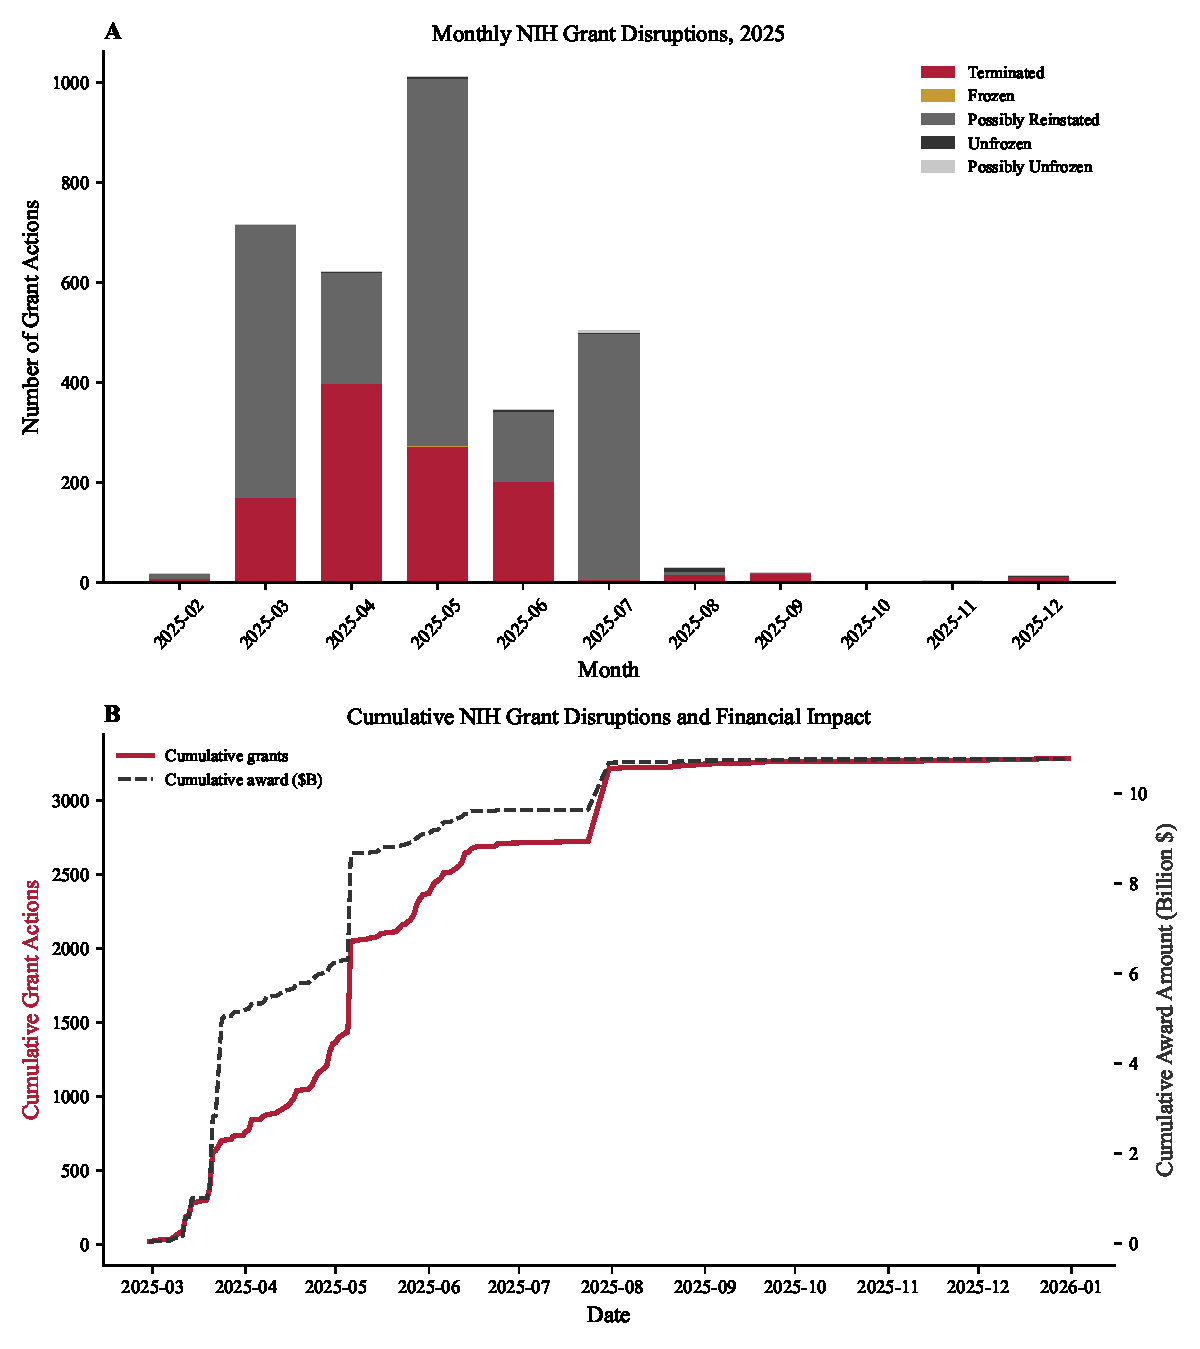
\includegraphics[width=\textwidth]{figure1.pdf}
\caption{Monthly Distribution and Cumulative Financial Impact of NIH Grant Disruptions, 2025.
Panel A shows the monthly count of grant actions by disruption status from January 2025 through early 2026. Panel B displays cumulative grant actions (left axis, crimson line) and cumulative obligated award amounts in billions of US dollars (right axis, dark gray dashed line) over the same period. The sharp rise in March 2025 corresponds to the first major wave of HHS-reported terminations.}
\label{fig:figure1}
\end{figure}

\begin{figure}[H]
\centering
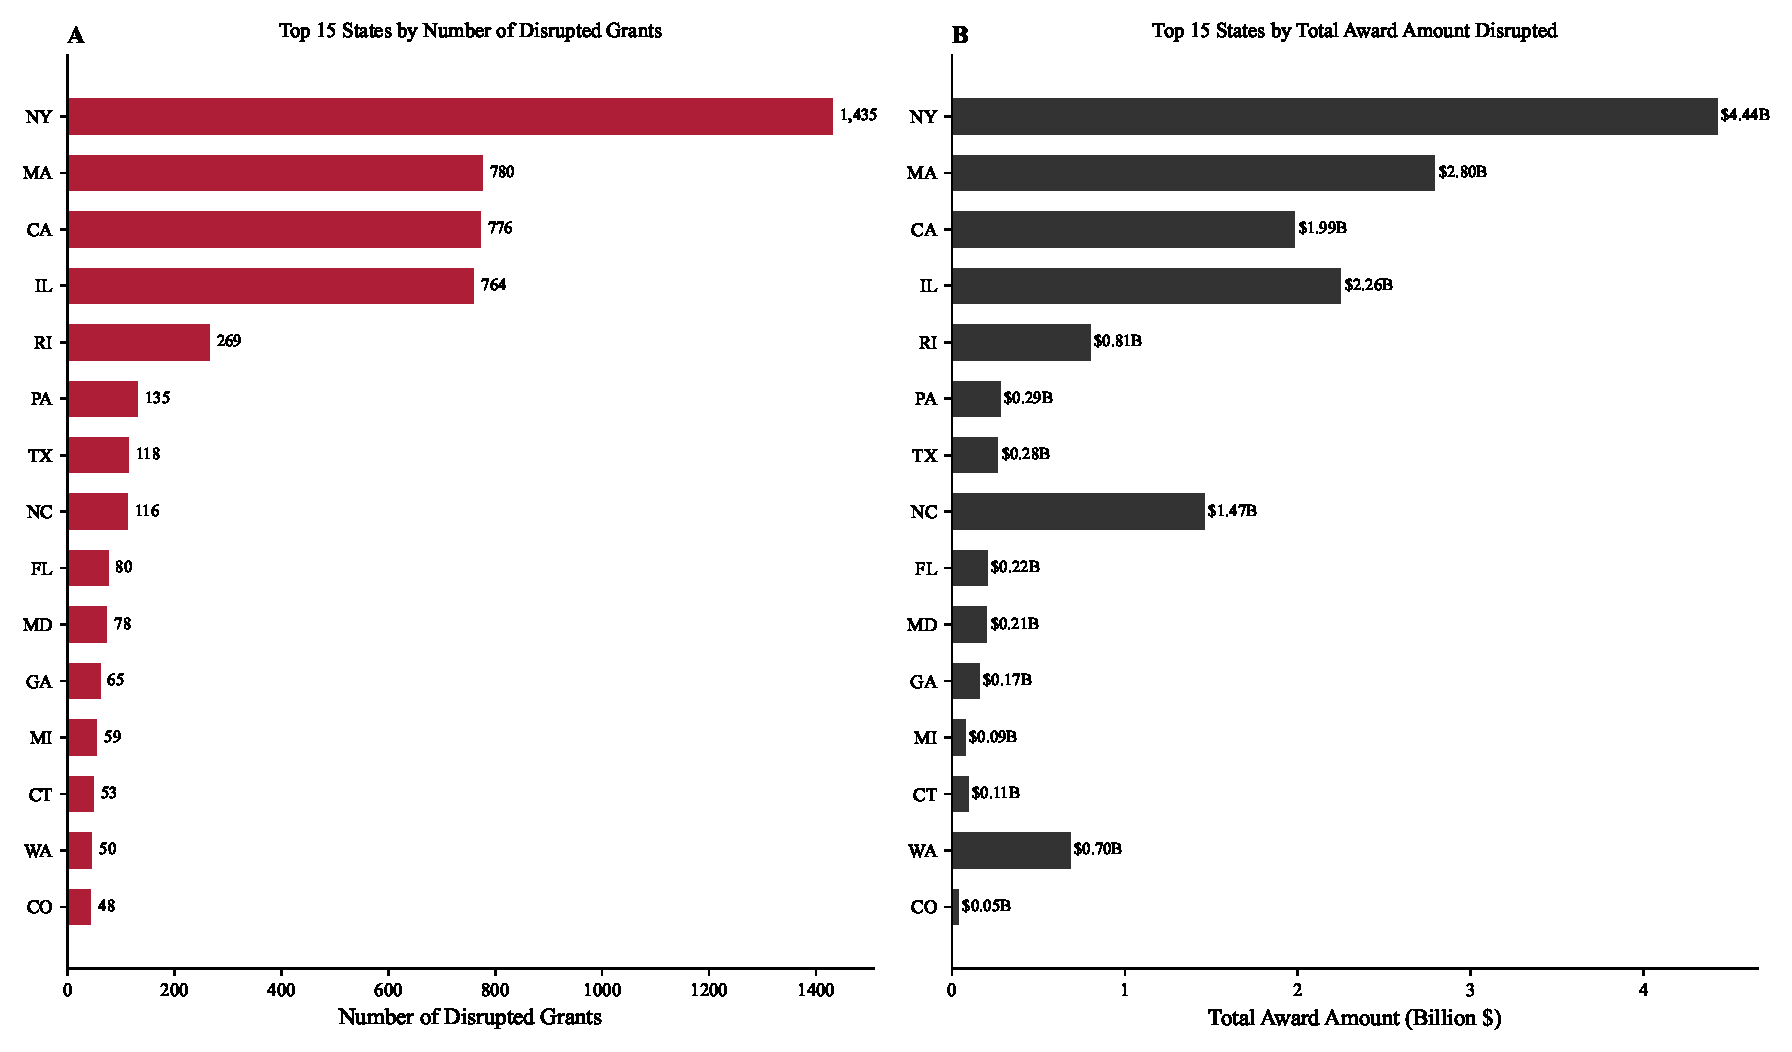
\includegraphics[width=\textwidth]{figure2.pdf}
\caption{Geographic Distribution of NIH Grant Disruptions by State, 2025.
Panel A shows the 15 states with the highest number of disrupted grants. Panel B shows the same 15 states ranked by total obligated award amount disrupted. New York, Massachusetts, and California dominate both measures, reflecting the concentration of major research universities and academic medical centers in these states.}
\label{fig:figure2}
\end{figure}

\begin{figure}[H]
\centering
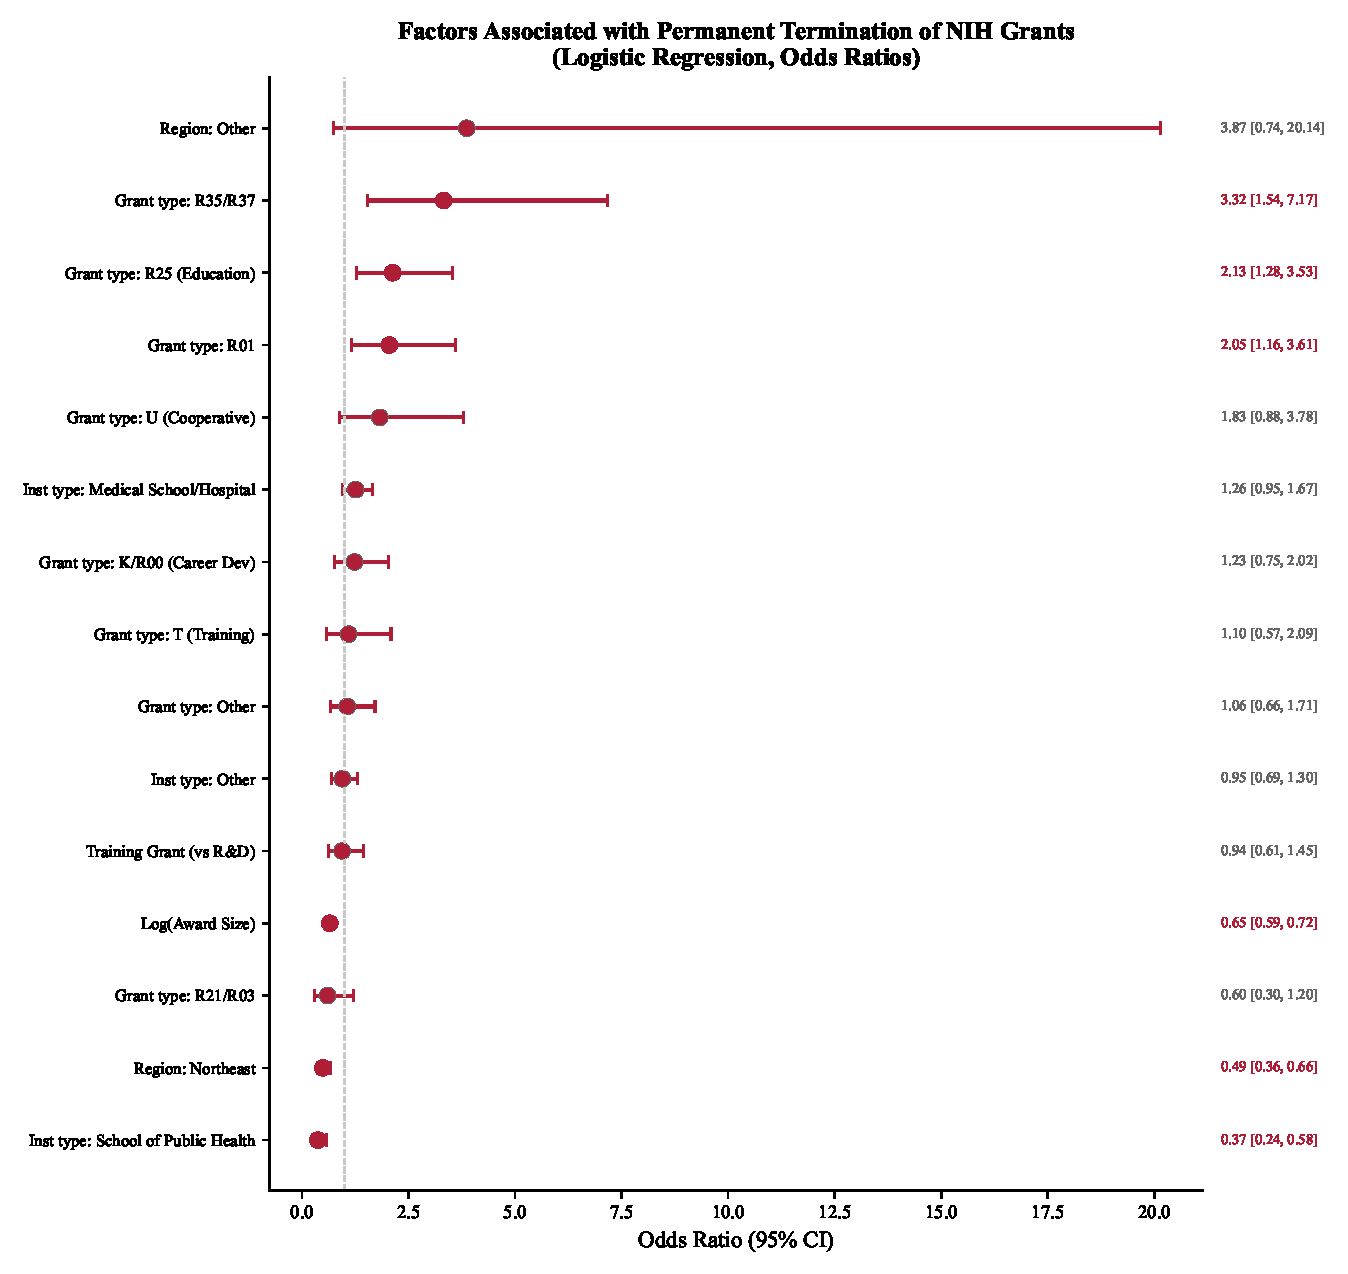
\includegraphics[width=0.9\textwidth]{figure3.pdf}
\caption{Factors Associated with Permanent Termination of NIH Grants: Multivariable Logistic Regression Results.
Forest plot of odds ratios (ORs) and 95\% confidence intervals from multivariable logistic regression (N~=~5\,400). OR~>~1 indicates higher odds of permanent termination; OR~<~1 indicates lower odds. Red dots indicate variables with \textit{P}~<~.05; gray dots indicate non-significant associations. The reference categories are F-series fellowship grants, Arts \& Sciences/University institutions, and Midwest region.}
\label{fig:figure3}
\end{figure}

\begin{figure}[H]
\centering
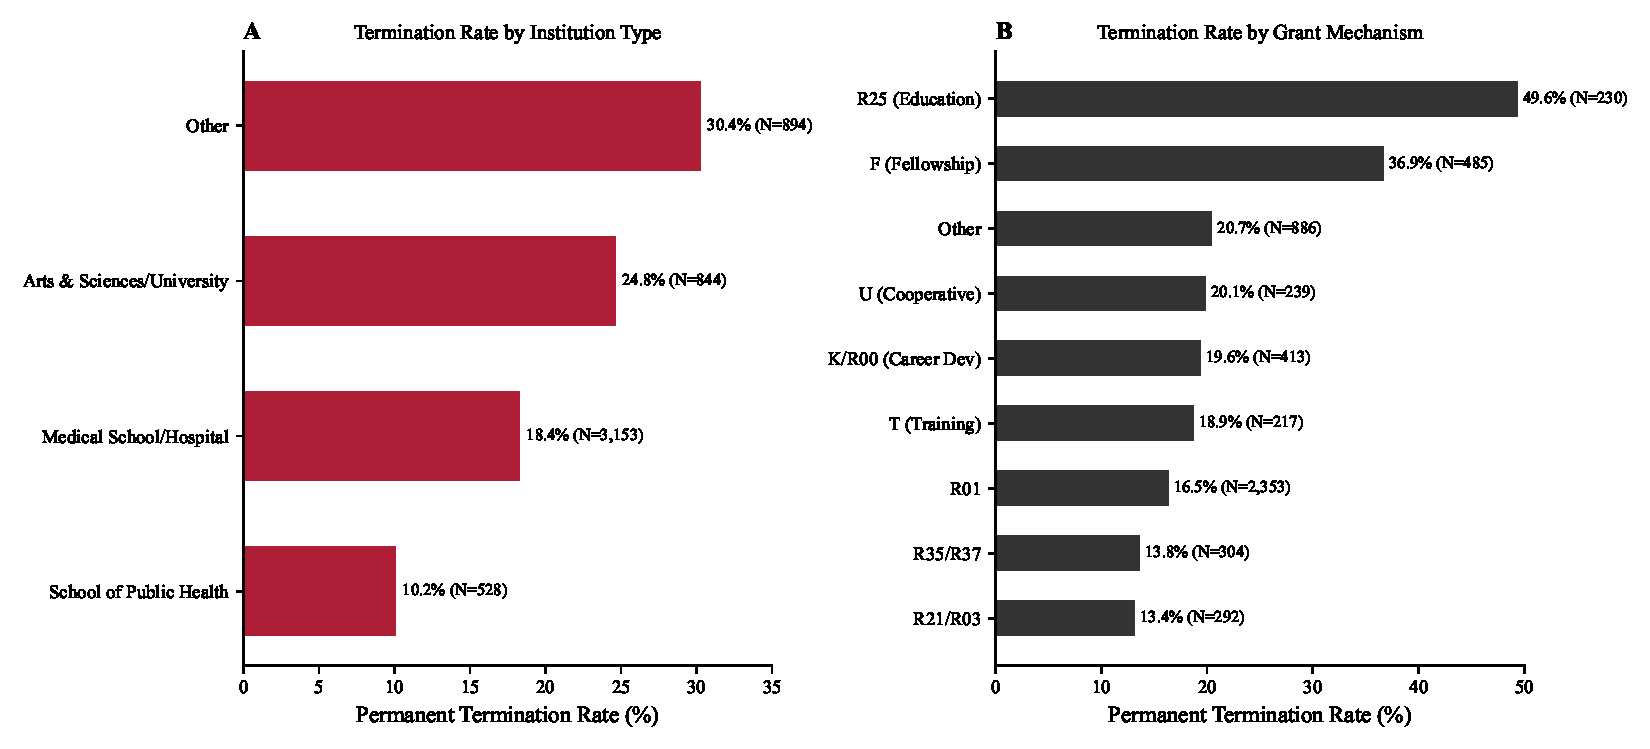
\includegraphics[width=\textwidth]{figure4.pdf}
\caption{Termination Rates by Institution Type and Grant Mechanism.
Panel A shows the proportion of grants receiving permanent termination by institution type (N within each category shown in parentheses). Panel B shows termination rates by NIH grant mechanism (activity code group). Bars represent the proportion of grants with that characteristic that received permanent termination status. R25 science education grants and F-series fellowships had the highest termination rates; Schools of Public Health had the lowest institutional termination rate.}
\label{fig:figure4}
\end{figure}


%% =============================================================================
%%  DISCUSSION
%% =============================================================================
\section*{Discussion}

In this cross-sectional analysis of 5\,419 disrupted NIH grants representing \$17.18 billion in total obligated awards, we found that the 2025 wave of federal research funding disruptions was not uniformly distributed but followed systematic patterns reflecting both policy priorities and the effectiveness of judicial intervention. Permanent terminations affected 1\,116 grants (20.6\%) worth \$1.73 billion in obligated funding, while the majority of disrupted awards---4\,283 (79.0\%)---were reinstated or unfrozen, predominantly through court-ordered stays and injunctions. These findings provide the first comprehensive cross-sectional characterization of the 2025 NIH funding crisis and suggest that administrative targeting, not random policy application, shaped which grants were ultimately lost.

The strong association between smaller award size and higher odds of permanent termination is consistent with a strategic selection of targets that are less likely to attract institutional legal defense. Higher-value grants, such as R35/R37 outstanding investigator awards and large U-series cooperative agreements, represent significant investments by research universities and are more likely to be defended in court. Indeed, the 0\% termination rate among the 548 grants documented through court filings underscores the critical role that litigation played in reversing these disruptions.\cite{aaas2025court,sciencemag2025court} The inverse award-size gradient persisted across funding categories and institution types in subgroup analyses, suggesting this is a robust pattern rather than an artifact of institutional differences.

The extraordinarily high termination rates for R25 science education grants (49.6\%) and F-series fellowship grants (36.9\%) are consistent with prior reporting that the 2025 disruptions specifically targeted grants related to diversity, equity, and inclusion (DEI) programs and training initiatives for underrepresented groups in science.\cite{sciencemag2025dei,nature2025cuts} R25 grants fund science education programs, many of which are designed to increase participation of underrepresented minorities in biomedical research.\cite{nih2025r25} Similarly, F-series fellowships fund individual predoctoral and postdoctoral trainees, many of whom received termination notices based on flagged keywords in grant abstracts. This finding has profound implications for the long-term diversity and inclusivity of the US scientific workforce.\cite{teitelbaum2024diversity,watkins2019minority}

Geographic variation in termination outcomes likely reflects both the distribution of grant types across regions and the differential effectiveness of state-level legal responses. The Northeast's low termination rate (10.9\%) is explained in part by the concentration of grants affiliated with Massachusetts institutions---the site of the most publicized legal battle involving Harvard University and multiple consortium grants.\cite{harvardgazette2025funding} The West's remarkably low termination rate (10.8\%) suggests that Western states were particularly aggressive in seeking court remedies, consistent with California's broader pattern of legal challenges to federal executive actions.\cite{california2025legal} By contrast, the Southeast's 66.2\% termination rate may reflect fewer institutional resources for legal challenge and a different political climate around challenging federal administrative actions.\cite{blume2018funding}

The finding that the training grant indicator was not independently associated with termination odds in the fully adjusted model (OR, 0.94; \textit{P}~= .793), despite unadjusted termination rates nearly double those of research grants, suggests that grant mechanism (activity code) and award size---not the broad training/research distinction---are the primary predictors of termination after adjustment. This is an important nuance: the vulnerability of training grants to termination appears to operate through the specific grant mechanisms (F31 fellowships and R25 education grants) rather than the category as a whole.

\subsection*{Policy Implications}

These findings have several important implications for research funding policy and institutional strategy. First, the substantial reversal of disruptions through litigation (79.0\% of affected grants reinstated or unfrozen) demonstrates that judicial oversight remains an effective check on executive actions affecting the scientific enterprise, but this protection is not equally accessible across institutions. Second, the patterns of termination targeting smaller grants, training programs, and education awards suggest that research universities and funding agencies should prioritize proactive legal protections for exactly these types of awards in any future disruption scenario. Third, the concentration of disrupted awards in a small number of high-research-intensity states (New York, Massachusetts, California, Illinois) means that funding disruptions---even if partially reversed---create substantial administrative burden and research interruption costs that are not captured in termination statistics alone.\cite{jones2023nih} Fourth, the \$7.15 billion in estimated remaining funds across all disrupted grants represents research infrastructure and ongoing studies that were placed in administrative limbo for months, with potentially irreversible effects on longitudinal cohorts, clinical trials, and early-career scientist trajectories.\cite{blume2018funding,teitelbaum2024diversity}

\subsection*{Limitations}

This study has several limitations. First, the Grant Witness database, while the most comprehensive publicly available source of 2025 NIH disruption data, relies on volunteer curation and may lag official databases by days to weeks, potentially missing some records or misclassifying status for recently changed awards. Second, the status classifications (terminated, frozen, unfrozen, possibly reinstated) are assigned by curators based on available information and may not perfectly reflect final legal or administrative outcomes, particularly for grants classified as ``possibly'' reinstated. Third, our cross-sectional analysis cannot establish causal mechanisms for the observed patterns; selection into termination may reflect unmeasured factors such as the specific language of grant abstracts, institutional political relationships, or the personal discretion of administering NIH program officers. Fourth, this study does not capture the full costs of disruption, including the administrative burden, loss of laboratory infrastructure, workforce attrition, and research continuity harms that persist even for reinstated grants. Fifth, our financial estimates are based on total obligated award amounts, which may overstate true remaining exposure since some portion of funds may have already been disbursed before the disruption date.

Despite these limitations, this study offers the first comprehensive quantitative characterization of the 2025 NIH funding crisis, providing estimates that can inform ongoing policy discussions and institutional planning.


%% =============================================================================
%%  CONCLUSIONS
%% =============================================================================
\section*{Conclusions}

In this cross-sectional analysis of 5\,419 disrupted NIH grants representing \$17.18 billion in obligated awards, the 2025 federal funding disruptions permanently terminated 1\,116 grants (20.6\%; \$1.73 billion in obligated value) while 4\,283 (79.0\%) were reinstated or unfrozen, primarily through judicial intervention. Larger grants were significantly less likely to be permanently terminated (OR, 0.65; 95\% CI, 0.59--0.72; \textit{P}~< .001), while R25 science education grants, R35/R37 outstanding investigator awards, and grants in the Southeast and US territories faced substantially higher odds of termination. These findings demonstrate that the 2025 NIH funding disruptions were not uniformly applied but targeted specific grant types, institutions, and geographic regions in patterns consistent with the administration's stated policy priorities. Future research should examine the long-term consequences of these disruptions for research output, scientific workforce composition, and public health outcomes.


%% =============================================================================
%%  ARTICLE INFORMATION
%% =============================================================================
\vspace{6pt}
\noindent{\color{jamalightgray}\rule{\textwidth}{0.4pt}}
\vspace{4pt}

\noindent\textbf{Author Contributions:} Wang had full access to all the data in the study and takes responsibility for the integrity of the data and the accuracy of the data analysis.

\noindent\textbf{Conflict of Interest Disclosures:} None reported.

\noindent\textbf{Funding/Support:} No external funding was received for this study.

\noindent\textbf{Role of the Funder/Sponsor:} Not applicable.

\noindent\textbf{Data Availability:} The Grant Witness dataset is publicly available at \url{https://grantwatch.org}. Analysis code is available at \url{https://github.com/class-repo/midterm-project}.


%% =============================================================================
%%  REFERENCES
%% =============================================================================

{\fontsize{8.5}{10.5}\selectfont
\bibliographystyle{vancouver}
\bibliography{references}
}


%% =============================================================================
%%  SUPPLEMENT (starts on new page)
%% =============================================================================
\clearpage
\section*{Supplement 1}

\subsection*{eAppendix 1. Statistical Models and Methods Details}

\textbf{Primary Logistic Regression Model.}
The primary analysis estimated the odds of permanent grant termination using a multivariable logistic regression:

\[
\log\!\left(\frac{P(\text{terminated}_{i}=1)}{1-P(\text{terminated}_{i}=1)}\right) = \alpha + \beta_1 \log(\text{award}_{i}) + \beta_2 \text{training}_{i} + \boldsymbol{\gamma}'\mathbf{A}_{i} + \boldsymbol{\delta}'\mathbf{O}_{i} + \boldsymbol{\eta}'\mathbf{R}_{i} + \boldsymbol{\theta}'\mathbf{C}_{i} + \varepsilon_{i}
\]

where $\log(\text{award}_{i})$ is the natural log of total obligated award amount for grant $i$; $\text{training}_{i}$ is a binary indicator for Research Training and Career Development category; $\mathbf{A}_{i}$ is a vector of activity code group dummies (reference: F-series fellowship); $\mathbf{O}_{i}$ is a vector of institution type dummies (reference: Arts \& Sciences/University); $\mathbf{R}_{i}$ is a vector of geographic region dummies (reference: Midwest); and $\mathbf{C}_{i}$ is a vector of cancellation source dummies (reference: Unknown). Results are reported as odds ratios (OR = $e^{\beta}$) with 95\% confidence intervals.

\textbf{Robustness Check: OLS on Log Remaining Funds.}
As a secondary analysis, we estimated an OLS regression on the natural log of estimated remaining funds:

\[
\log(\text{remaining}_{i}) = \alpha + \beta_1 \log(\text{award}_{i}) + \beta_2 \text{training}_{i} + \boldsymbol{\gamma}'\mathbf{A}_{i} + \boldsymbol{\delta}'\mathbf{O}_{i} + \boldsymbol{\eta}'\mathbf{R}_{i} + \varepsilon_{i}
\]

Standard errors were estimated using the HC1 heteroskedasticity-robust estimator.\cite{white1980het}

\subsection*{eTable 1. Top 15 States by Number of Disrupted NIH Grants, 2025}

\begin{table}[H]
\centering
\sffamily\fontsize{8.5}{11}\selectfont
\begin{tabular}{lrrrr}
\toprule
\textbf{State} & \textbf{Total Grants} & \textbf{Terminated} & \textbf{Term.\ Rate (\%)} & \textbf{Total Award (\$B)} \\
\midrule
New York       & 1,435 & 74  & 5.2  & 4.81 \\
Massachusetts  & 780   & 36  & 4.6  & 3.88 \\
California     & 776   & 75  & 9.7  & 1.91 \\
Illinois       & 764   & 16  & 2.1  & 1.01 \\
Rhode Island   & 269   & 2   & 0.7  & 0.40 \\
Pennsylvania   & 135   & 27  & 20.0 & 0.37 \\
Texas          & 118   & 95  & 80.5 & 0.28 \\
North Carolina & 116   & 71  & 61.2 & 0.26 \\
Florida        & 80    & 78  & 97.5 & 0.20 \\
Maryland       & 78    & 45  & 57.7 & 0.24 \\
Washington     & 70    & 7   & 10.0 & 0.28 \\
Ohio           & 69    & 36  & 52.2 & 0.15 \\
Michigan       & 68    & 16  & 23.5 & 0.16 \\
Wisconsin      & 64    & 17  & 26.6 & 0.17 \\
Minnesota      & 61    & 8   & 13.1 & 0.18 \\
\bottomrule
\end{tabular}
\caption{Top 15 states by number of disrupted grants. Termination rate reflects the proportion of disrupted grants in each state that received permanent termination status. Southern states (Texas, Florida, North Carolina) show markedly higher termination rates than Northeastern and Western states.}
\end{table}

\subsection*{eFigure 1. Termination Rate by Institution Type and Grant Mechanism}

See Figure~4 in the main text.

\subsection*{eTable 2. Complete Logistic Regression Results}

\begin{table}[H]
\centering
\sffamily\fontsize{8}{10}\selectfont
\begin{tabular}{lrrrr}
\toprule
\textbf{Variable} & \textbf{OR} & \textbf{95\% CI} & \textbf{\textit{P} Value} \\
\midrule
Log(Total Award)         & 0.65 & 0.59--0.72 & $<$.001 \\
Training Grant (vs.\ R\&D) & 0.94 & 0.61--1.45 & .793 \\
Activity: R01            & 2.05 & 1.16--3.61 & .013 \\
Activity: R25 Education  & 2.13 & 1.28--3.53 & .003 \\
Activity: R35/R37        & 3.32 & 1.54--7.17 & .002 \\
Activity: R21/R03        & 0.60 & 0.30--1.20 & .149 \\
Activity: K/R00          & 1.23 & 0.75--2.02 & .404 \\
Activity: U Cooperative  & 1.83 & 0.88--3.78 & .104 \\
Activity: Other          & 1.06 & 0.66--1.71 & .801 \\
Inst: Medical School     & 1.26 & 0.95--1.67 & .104 \\
Inst: Public Health      & 0.37 & 0.24--0.58 & $<$.001 \\
Inst: Other              & 0.95 & 0.69--1.30 & .743 \\
Region: Northeast        & 0.49 & 0.36--0.66 & $<$.001 \\
Region: Southeast        & 1.19 & 0.86--1.65 & .286 \\
Region: West             & 0.12 & 0.08--0.17 & $<$.001 \\
Region: Other/Territory  & 3.75 & 2.13--6.61 & $<$.001 \\
\bottomrule
\end{tabular}
\caption{Complete adjusted logistic regression results. OR = odds ratio; CI = confidence interval. Reference categories: F-series fellowship (activity code), Arts \& Sciences/University (institution type), Midwest (region). N = 5,400.}
\end{table}


\end{document}
